\section{PS4a: CircularBuffer}\label{sec:ps4a}

\subsection{Discussion}\label{sec:ps4a:disc}

This project is to prepare a header file for ps4b.
we have to store a data into the container and use it for later.
I used vector to store the datas because I am used to it. I used this for 2 other projects.
For member variables I have 5 because we need vector to store, beg to find out the first vector, end for the last, and si for size of the vector and cap for capacity of the vector.

\begin{figure}[tbh]
	\centering
	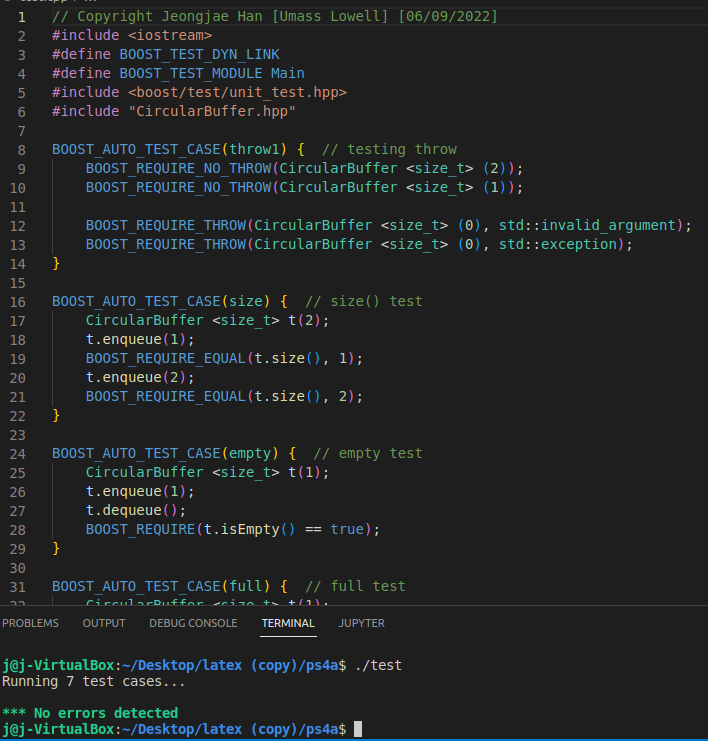
\includegraphics[width=10cm]{ps4a}
	\caption{Testing CircularBuffer.hpp}
	\label{fig:ps4a}
\end{figure}

I made tests for all the functions I have for headerfile : Constructor, size(), isEmpty(), isFull(), peek(), enqueue(T item), and dequeue().
For exceptions I used invalid-argument and run-time error and the code throws the exceptions properly.

For the complexity for my CircularBuffer, it is O(1), since I have the member variable for begin and end, so it can be used as index.

\subsection{Places to get help}
I got help from: Lecture slide: template, stackoverflow, youtube.

%\subsection{What I accomplished}\label{sec:ps0:accomplish}

%\subsection{What I already knew}\label{sec:ps0:knew}

\subsection{What I learned}\label{sec:ps4a:learned}

I also learned how to use the vector as private member variable. I was having hard time putting vector container as private member variable for previous projects.

For the construct argument, due to the type sizeT, negative value cannot be passed, so I tried to figure out how to throw an exception, but could not find out anywhere.

\subsection{Challenges}\label{sec:ps4a:challenges}

I got used to using template more and for the constructor with this project. I have to declare argument's original datatype to pass it properly. It took a while to find it out.

\subsection{Mistakes}\label{sec:ps4a:mistakes}

I got one point off because my program has incorrect behavior when interleaving enqueue and dequeue operation.

\subsection{Codebase}\label{sec:ps4a:code}
Makefile
\lstinputlisting[language=Make]{ps4a/Makefile}
CircularBuffer.hpp
\lstinputlisting{ps4a/CircularBuffer.hpp}
test.cpp
\lstinputlisting{ps4a/test.cpp}

\newpage
